\documentclass[11pt,a4paper]{article}
\usepackage[margin=24mm]{geometry}
\usepackage[T1]{fontenc}
\usepackage[utf8]{inputenc}
\usepackage{lmodern}
\usepackage{microtype}
\usepackage{amsmath,amssymb,amsthm}
\usepackage{booktabs,longtable,tabularx,array}
\usepackage{graphicx,xcolor,tikz}
\usetikzlibrary{arrows.meta,positioning,calc}
\usepackage{enumitem,fancyhdr,listings}
\usepackage{caption}
\usepackage{hyperref}

\definecolor{ink}{HTML}{183247}
\definecolor{teal}{HTML}{168C88}
\definecolor{blue}{HTML}{2B5D89}
\definecolor{light}{HTML}{F1F6F6}
\definecolor{paper}{HTML}{F2F5F8}
\definecolor{muted}{HTML}{536875}
\hypersetup{colorlinks=true,linkcolor=blue,urlcolor=blue,citecolor=blue,
  pdftitle={Simplifying Numerical PDE Algorithms: Sections 1, 2 and 4},
  pdfauthor={Team iberIAn\_solvers},
  pdfsubject={Green functions, the FFT, and butterfly factorisation}}
\pagestyle{fancy}
\fancyhf{}
\fancyhead[L]{\small Team iberIAn\_solvers · Problem 29}
\fancyhead[R]{\small Interim report: Sections 1, 2 and 4}
\fancyfoot[C]{\thepage}
\setlength{\headheight}{14pt}
\setlist{nosep,leftmargin=1.6em}
\renewcommand{\arraystretch}{1.16}
\setlength{\emergencystretch}{2em}
\setlength{\parskip}{0.2em}
\numberwithin{equation}{section}
\lstset{basicstyle=\ttfamily\footnotesize,breaklines=true,showstringspaces=false,
  frame=single,rulecolor=\color{black!20},backgroundcolor=\color{paper}}
\newcommand{\eps}{\varepsilon}
\newcommand{\dd}{\mathop{}\!\mathrm{d}}
\newcommand{\nnz}{\operatorname{nnz}}
\newcommand{\T}{\mathsf{T}}
\newcommand{\takeaway}[1]{\begin{center}\colorbox{light}{\parbox{0.94\linewidth}{\vspace{5pt}\centering\textbf{#1}\vspace{5pt}}}\end{center}}
\newenvironment{evidence}{\begin{quote}\small\color{muted}\textbf{Evidence status.} }{\end{quote}}

\title{\vspace{-8mm}\LARGE\bfseries Simplifying Numerical PDE Algorithms\\[5pt]
\Large From Green functions to the FFT and butterfly factorisation\\[4pt]
\large Interim report: Sections 1, 2 and 4}
\author{\Large\textbf{Team iberIAn\_solvers}\\[4pt]
\textbf{Problem 29: Simplifying PDE Algorithms}\\[4pt]
\url{https://github.com/carlesfalco/mathathon-iberIAn_solvers}}
\date{Caltech Mathathon · Round 1}

\begin{document}
\maketitle
\thispagestyle{fancy}

\begin{abstract}
\noindent
Fast numerical algorithms for partial differential equations often look complicated because several different kinds of structure are used at once. This interim report develops a continuous explanation through three of the project's sections. We first show how Green-function formulations turn PDEs into integral equations and dense, structured matrices. We then use the FFT to separate two ideas that are sometimes conflated: diagonalization of a periodic operator and sparse factorization of the Fourier basis change. Finally, we explain butterfly factorisation for oscillatory integral operators through centred phase subtraction, complementary boxes, low-rank blocks, and nested transfers.

The emphasis is on making the algorithms understandable without weakening the mathematics. Exact identities are derived, approximation claims are tied to explicit norms and assumptions, and numerical experiments are labelled separately from proofs. The FFT, butterfly algorithm, and their underlying principles are established work; the contribution here is a coordinated exposition and reproducible checks, not a new universal solver.
\end{abstract}

\noindent\textbf{Scope of this version.} This document currently merges the project's Sections~1,~2, and~4. Their original numbers are retained for consistency with the section drafts; Section~3 and the later sections will be integrated in subsequent versions. No result from an omitted section is required for the derivations below.

\tableofcontents
\clearpage


% ---- Original Section 1, adapted for this report ----
\section{Motivation: PDEs and Green-function integrals}
\label{sec:motivation}

Many numerical methods for partial differential equations (PDEs) lead, either directly or after an intermediate reformulation, to integrals of the form
\begin{equation}
    u(x) = \int_\Omega G(x,y) f(y)\,\mathrm{d}y.
    \label{eq:green-representation}
\end{equation}
Here, $f$ represents a source or given data, $u$ is the quantity to be computed, and $G$ is a \emph{Green function}. The value $G(x,y)$ describes the effect at an observation point $x$ of a unit point source located at $y$. Equation~\eqref{eq:green-representation} therefore expresses a superposition principle: the solution at $x$ receives contributions from sources throughout the domain.

After discretization, such integral operators become matrices. Their properties depend on the PDE, the geometry, and the chosen formulation: a matrix may be diagonal in a suitable basis, sparse, translation invariant, or dense and oscillatory. Understanding and exploiting this structure is the common theme of the methods studied in this report.

\subsection{Green functions and linear systems}

Consider a linear PDE written abstractly as $\mathcal{L}u=f$ in $\Omega$, together with suitable homogeneous boundary or initial conditions. Its Green function formally satisfies
\begin{equation}
    \mathcal{L}_xG(x,y)=\delta(x-y),
\end{equation}
with the same homogeneous conditions in $x$, where $\delta$ is the Dirac distribution. Applying $\mathcal{L}$ to~\eqref{eq:green-representation} then recovers $\mathcal{L}u=f$. Other boundary or initial data introduce additional terms without changing this basic representation.

When pointwise quadrature is applicable, choosing source points $y_j$, observation points $x_i$, and quadrature weights $w_j$ gives
\begin{equation}
    u(x_i)\approx\sum_{j=1}^{N}w_jG(x_i,y_j)f(y_j)
    =\sum_{j=1}^{N}A_{ij}f_j,
    \qquad A_{ij}=w_jG(x_i,y_j).
    \label{eq:discrete-green}
\end{equation}
Thus, a continuous integral operator becomes the matrix operation $u=Af$. More generally, an integral equation constrains the unknown itself, and discretization produces a linear system
\begin{equation}
    A\sigma=b
    \label{eq:generic-system}
\end{equation}
whose solution is needed before physical quantities can be recovered.

These are two distinct numerical tasks. \emph{Applying} an operator means computing $A\sigma$ for a given $\sigma$, whereas \emph{solving} a system means finding $\sigma$ from $A\sigma=b$. A fast method for the first task does not automatically provide a fast method for the second. Fast direct solvers address the second task by constructing a reusable representation of the solution operator.

For an unstructured $N\times N$ matrix, the usual baselines are
\begin{center}
\begin{tabular}{@{}ll@{}}
Operation & Standard dense cost \\
\hline
Storing $A$ & $O(N^2)$ memory \\
Applying $Af$ & $O(N^2)$ operations \\
Computing an LU factorization & $O(N^3)$ operations \\
Solving using stored LU factors & $O(N^2)$ operations per right-hand side
\end{tabular}
\end{center}
Evaluating a kernel sum directly does not require storing the full matrix, because its entries can be generated when needed, but a direct evaluation still involves $N^2$ kernel interactions. These generic costs motivate the search for specialized representations and factorizations.

\subsection{An explicit example: a one-dimensional reaction--diffusion problem}
\label{subsec:reaction-diffusion}

To see how an actual equation leads to a system of the form~\eqref{eq:generic-system}, consider the steady reaction--diffusion problem
\begin{equation}
    -u''(x)+q(x)u(x)=f(x),\qquad 0<x<1,
    \qquad u(0)=u(1)=0.
    \label{eq:reaction-diffusion}
\end{equation}
Here, $q$ is a given nonnegative coefficient and $f$ is a known source. If $q$ varies with $x$, the reaction term couples different Fourier modes, so the equation generally does not reduce to independent scalar equations in a simple global Fourier basis.

First consider the background operator $-d^2/dx^2$ with the same Dirichlet conditions. Its Green function is
\begin{equation}
    G_0(x,y)=
    \begin{cases}
        x(1-y), & 0\leq x\leq y\leq1,\\
        y(1-x), & 0\leq y<x\leq1.
    \end{cases}
    \label{eq:dirichlet-green}
\end{equation}
Indeed, $G_0$ is continuous, satisfies the boundary conditions in $x$, and has the derivative jump required to produce $\delta(x-y)$ under $-\partial_{xx}$. Define the known function
\begin{equation}
    F(x)=\int_0^1G_0(x,y)f(y)\,\mathrm{d}y.
    \label{eq:reaction-source}
\end{equation}
Since $-u''=f-qu$, applying the background Green operator gives
\begin{equation}
    u(x)+\int_0^1G_0(x,y)q(y)u(y)\,\mathrm{d}y=F(x).
    \label{eq:reaction-integral}
\end{equation}
The unknown $u$ now appears on both sides of the equation. It is no longer sufficient to evaluate one Green-function integral with known data; we must solve an integral equation.

After quadrature, equation~\eqref{eq:reaction-integral} becomes
\begin{equation}
    u_i+\sum_{j=1}^{N}w_jG_0(x_i,x_j)q(x_j)u_j=F_i,
    \qquad i=1,\ldots,N,
    \label{eq:reaction-discrete-sum}
\end{equation}
or, in matrix notation,
\begin{equation}
    (I+KQ)u=F,
    \qquad K_{ij}=w_jG_0(x_i,x_j),
    \qquad Q=\operatorname{diag}(q(x_1),\ldots,q(x_N)).
    \label{eq:reaction-system}
\end{equation}
The matrix $K$, and hence generally $I+KQ$, is dense because every source point contributes to every observation point. At the same time, its entries are samples of a simple Green kernel rather than unrelated numbers.

Importantly, this example needs no singular-diagonal correction: $G_0$ is continuous everywhere and
\begin{equation}
    G_0(x,x)=x(1-x)
    \label{eq:green-diagonal}
\end{equation}
is finite. Thus, the formula $K_{ij}=w_jG_0(x_i,x_j)$ remains meaningful when $i=j$.

The example also shows that the matrix structure depends on the formulation. A local finite-difference discretization of~\eqref{eq:reaction-diffusion} leads to a sparse system, whereas the Green formulation leads to a dense one. The integral formulation is not automatically preferable for this one-dimensional problem; it serves here to demonstrate how PDEs produce dense integral-operator systems and why different algebraic structures require different algorithms.

\subsection{From examples to structured matrix problems}

This reaction--diffusion problem illustrates the central computational question: how can we represent and solve a large matrix system efficiently by using the structure inherited from the PDE? Periodic evolution problems provide cases that become diagonal in Fourier space; local differential discretizations provide sparse systems; and oscillatory Green or Fourier integral operators provide dense matrices with more subtle interaction patterns. The following sections examine these structures separately, beginning with the most regular ones and progressing toward oscillatory operators and their factorizations.

% ---- Original Section 2, adapted for this report ----
\section{The FFT: exact structure and sparse stages}
\label{sec:fft}

Section~1 allows a general dense Green matrix. We now impose enough symmetry to obtain an exact fast method. The point is not merely that Fourier modes diagonalize a periodic operator: the changes of basis must also be cheap.

\subsection{Circulant interactions become diagonal in Fourier variables}
Suppose a discrete integral operator has the translation-invariant form
\begin{equation}
 (Kf)_i=\sum_{j=0}^{N-1}g_{(i-j)\bmod N}f_j,
 \qquad 0\le i<N.
 \label{eq:circulant}
\end{equation}
The matrix $K$ is \emph{circulant}: every row is a cyclic shift of the previous one. This structure comes from the kernel, grid, weights, and periodic boundary conditions together; an irregular boundary does not generally possess it.

For $v^{(k)}_j=e^{2\pi ikj/N}$, substitution of $\ell=i-j$ gives
\begin{equation}
 (Kv^{(k)})_i=v^{(k)}_i\mu_k,
 \qquad
 \mu_k=\sum_{\ell=0}^{N-1}g_\ell e^{-2\pi ik\ell/N}.
 \label{eq:circulant-eigen}
\end{equation}
Define the unitary DFT by
\begin{equation}
 (\mathcal F_N)_{kj}=N^{-1/2}e^{-2\pi ikj/N},
 \qquad \widehat f=\mathcal F_Nf.
 \label{eq:unitary-dft}
\end{equation}
The geometric-sum identity proves $\mathcal F_N^*\mathcal F_N=I$, and~\eqref{eq:circulant-eigen} becomes the exact matrix identity
\begin{equation}
 K=\mathcal F_N^*\operatorname{diag}(\mu)\mathcal F_N,
 \qquad \mu=\sqrt N\,\mathcal F_Ng.
 \label{eq:circulant-factor}
\end{equation}
\begin{evidence}
The mode calculation and orthogonality sum prove~\eqref{eq:circulant-factor} exactly for every $N$; this is not a numerical approximation.
\end{evidence}

\subsection{Radix-2 recursion makes the basis change fast}
Assume $N=2^L$ and temporarily use the unnormalized transform $X=\sqrt N\,\mathcal F_Nx$. Put $\omega_N=e^{-2\pi i/N}$ and separate even and odd input indices:
\begin{align}
 X_k&=\sum_{r=0}^{N/2-1}x_{2r}\omega_{N/2}^{rk}
      +\omega_N^k\sum_{r=0}^{N/2-1}x_{2r+1}\omega_{N/2}^{rk}
      =E_k+\omega_N^kO_k,\\
 X_{k+N/2}&=E_k-\omega_N^kO_k,
 \qquad 0\le k<N/2.
 \label{eq:cooley-tukey}
\end{align}
Here $E$ and $O$ are length-$N/2$ transforms. Their values repeat after $N/2$, while $\omega_N^{k+N/2}=-\omega_N^k$. Thus the same two partial sums produce two outputs. No term is discarded; the two-input/two-output recombination is called a \emph{butterfly}.

For example, when $x=(1,2,3,4)$, the even and odd transforms are $E=(4,-2)$ and $O=(6,-2)$. Since $\omega_4=-i$, the two output pairs combine to
\begin{equation}
 X=(10,-2+2i,-2,-2-2i).
\end{equation}
This is exactly the dense four-point transform, obtained by reusing the two partial sums rather than discarding information.

In matrix form, let $P_N$ be the even-before-odd permutation and set $D_N=\operatorname{diag}(\omega_N^k)_{k=0}^{N/2-1}$. Then
\begin{equation}
 \mathcal F_N=
 \underbrace{\frac1{\sqrt2}
 \begin{bmatrix}I&D_N\\I&-D_N\end{bmatrix}}_{\text{sparse combination}}
 \begin{bmatrix}\mathcal F_{N/2}&0\\0&\mathcal F_{N/2}\end{bmatrix}
 \underbrace{P_N}_{\text{reordering}}.
 \label{eq:fft-step}
\end{equation}
Iterating to scalar transforms gives $L=\log_2N$ sparse combination stages and a bit-reversal permutation:
\begin{equation}
 \mathcal F_N=S_LS_{L-1}\cdots S_1\Pi_N.
 \label{eq:fft-stages}
\end{equation}
Each stage has $2N$ nonzero entries. Equivalently, the algorithmic recurrence is
\[
 T(N)=2T(N/2)+O(N)=O(N\log N).
\]
This is the classical Cooley--Tukey factorization~\cite{cooley1965fft}. An in-place implementation does not materialize $S_\ell$ or $\mathcal F_N$.
\takeaway{Diagonalization and fast basis changes are separate steps; the FFT solver needs both.}

\subsection{A periodic discrete Green operator}
Consider the companion to Section~\ref{subsec:reaction-diffusion} with constant reaction and periodic conditions:
\begin{equation}
 -u''+u=f,\qquad x\in[0,1],\qquad u(0)=u(1),\quad u'(0)=u'(1).
 \label{eq:periodic-pde}
\end{equation}
For $N=2^L\ge4$, on $x_j=jh$, $h=1/N$, use centered differences with indices modulo $N$. To avoid confusing the sparse differential matrix with the dense matrices $A$ and $K$ elsewhere, write
\begin{equation}
 (Su)_j=u_j-\frac{u_{j+1}-2u_j+u_{j-1}}{h^2}=f_j,
 \qquad S=I-\Delta_h.
 \label{eq:periodic-stencil}
\end{equation}
Substitution of $v^{(k)}$ gives
\begin{equation}
 S=\mathcal F_N^*\Lambda\mathcal F_N,
 \qquad
 \lambda_k=1+\frac4{h^2}\sin^2\!\left(\frac{\pi k}{N}\right),\qquad
 \Lambda=\operatorname{diag}(\lambda_0,\ldots,\lambda_{N-1}).
 \label{eq:periodic-symbol}
\end{equation}
Since $\lambda_k\ge1$, inversion is well defined and the discrete Green operator is
\begin{equation}
 G_h:=S^{-1}=\mathcal F_N^*\Lambda^{-1}\mathcal F_N.
 \label{eq:periodic-green}
\end{equation}
To solve $Su=f$, one applies the two FFTs and divides the $N$ Fourier coefficients by $\lambda_k$. The work is $O(N\log N)$ and standard working storage is $O(N)$; neither $G_h$ nor $\mathcal F_N$ is formed. The continuous Fourier eigenvalue $1+4\pi^2k^2$ has been replaced by the correct discrete symbol in~\eqref{eq:periodic-symbol}.

For even $N$, the displayed spectrum also gives $\kappa_2(S)=\lambda_{N/2}/\lambda_0=1+4N^2$. Well-defined inversion therefore does not mean conditioning is uniform in $N$. Dropping the reaction term would additionally make $\lambda_0=0$, requiring compatibility of $f$ and a convention for the mean of $u$.

\subsection{Checked algebra versus PDE error}
\label{sec:fft-checks}
The script \path{consolidated/examples/fft_periodic_solver.py} independently constructs $S$ and $\mathcal F_N$, checks the sparse-stage product~\eqref{eq:fft-stages}, compares a recursive radix-2 transform against the dense DFT on deterministic complex inputs, and compares the FFT solve with a dense solve. Table~\ref{tab:fft-algebra} reports locally rerun double-precision results using Python 3.12.14 and NumPy 2.5.3. The matrix norm is Frobenius and vector norms are Euclidean.
\begin{table}[htbp]
\centering\small
\caption{Local algebraic checks for $N=8,16,32,64$. The three columns are respectively $\|S-\mathcal F_N^*\Lambda\mathcal F_N\|_F/\|S\|_F$, FFT-versus-dense solution error, and relative residual. These finite checks complement, rather than replace, the exact derivations.}
\label{tab:fft-algebra}
\begin{tabular}{@{}rrrr@{}}
\toprule
$N$ & Factorization error & Solve error & Relative residual \\
\midrule
8  & $8.59\times10^{-16}$ & $2.71\times10^{-15}$ & $4.57\times10^{-16}$\\
16 & $2.18\times10^{-15}$ & $1.01\times10^{-14}$ & $2.36\times10^{-15}$\\
32 & $3.74\times10^{-15}$ & $5.36\times10^{-15}$ & $6.89\times10^{-15}$\\
64 & $7.98\times10^{-15}$ & $2.31\times10^{-14}$ & $2.99\times10^{-14}$\\
\bottomrule
\end{tabular}
\end{table}

Over the same sizes, the largest unitary defect was $8.97\times10^{-15}$, the largest sparse-stage reconstruction error $8.10\times10^{-15}$, and the largest recursive-FFT error $7.00\times10^{-15}$. All three are below the script's $10^{-12}$ verification threshold.

A separate computation samples the continuum forcing associated with $u_\star(x)=\cos(2\pi x)+\tfrac15\sin(4\pi x)$ and compares the discrete solution with samples of $u_\star$:
\begin{center}
\begin{tabular}{@{}rrrrr@{}}
\toprule
$N$ & 16 & 32 & 64 & 128\\
\midrule
Relative discretization error & $1.613\times10^{-2}$ & $3.980\times10^{-3}$ & $9.920\times10^{-4}$ & $2.478\times10^{-4}$\\
\bottomrule
\end{tabular}
\end{center}
Successive error ratios are $4.051$, $4.013$, and $4.003$. For each fixed mode, Taylor expansion of~\eqref{eq:periodic-symbol} gives
\[
 1+4h^{-2}\sin^2(\pi kh)
 =1+4\pi^2k^2-\frac43\pi^4k^4h^2+O(h^4),
\]
which explains the observed second-order convergence. The FFT accelerates the discrete solve; it does not remove finite-difference error or resolve frequencies absent from the grid.
\begin{evidence}
Equations~\eqref{eq:periodic-symbol}--\eqref{eq:periodic-green} are proved by substitution. The numerical tables are locally rerun computations over exactly the displayed sizes, with output in \path{consolidated/results/local/}; they are not general forward-error guarantees or timing benchmarks.
\end{evidence}

\subsection{What generalizes---and what does not}
The quadratic baseline is dense application of $G_h=S^{-1}$, not application of the sparse stencil $S$. For this one-dimensional periodic problem, specialized cyclic-tridiagonal solvers can be asymptotically cheaper than an FFT; the FFT is our canonical explanation of structured computation, not a claim of optimality for every constant-coefficient 1-D problem.

Most importantly, fast application does not imply that the full matrix is approximately low rank. Since $\mathcal F_N$ is unitary, every singular value equals one. If $R$ has rank less than $N$, choose a unit vector $z\in\ker R$. Then
\begin{equation}
 \|(\mathcal F_N-R)z\|_2=\|\mathcal F_Nz\|_2=1,
 \qquad\text{so}\qquad \|\mathcal F_N-R\|_2\ge1.
 \label{eq:fft-full-rank}
\end{equation}
Thus no relative spectral approximation of the whole Fourier matrix at small tolerance has low rank. Its speed comes from the sparse product~\eqref{eq:fft-stages}.

The broader design objective is therefore
\begin{equation}
 A\approx \widetilde A=T_MT_{M-1}\cdots T_1P,
 \qquad\text{each }T_\ell\text{ inexpensive to apply}.
 \label{eq:factor-design}
\end{equation}
If $M=O(\log N)$ and each stage costs $O(N)$, application costs $O(N\log N)$. Existence, accuracy, construction cost, and stability must be established separately. For oscillatory operators without exact Fourier symmetry, butterfly factorization supplies one such route; for direct solves, elimination adds further stability questions.

% Keep the source draft number: Section 3 is intentionally not in this version.
\setcounter{section}{3}
% ---- Original Section 4, adapted for this report ----
\section{The butterfly factorisation for oscillatory integral operators}
\label{sec:butterfly}

Discrete Fourier integral operators (FIOs) have dense, oscillatory matrices, so a direct matrix--vector product is expensive. The butterfly algorithm obtains a faster representation by using low-rank approximations on specially chosen blocks. For the FIOs considered by Cand\`{e}s, Demanet, and Ying, these blocks and their accuracy can be understood through a centred expansion of the phase~\cite{candes2009butterfly}.

We first explain the mechanism in one dimension. Consider the oscillatory kernel
\begin{equation}
    K_n(x,p)=e^{2\pi i n\Psi(x,p)},
    \label{eq:scaled-kernel}
\end{equation}
where $\Psi$ is real and smooth. The parameter $n$ measures the frequency scale; it will also determine the depth of the block partition. The one-dimensional notation is simpler than that of the paper, but the essential estimate is unchanged.

\subsection{The centred rectangle expansion}

Let $A$ and $B$ be intervals of widths $h_A$ and $h_B$, centred at $a$ and $b$. On the rectangle $A\times B$, define the double difference
\begin{equation}
    R_{AB}(x,p)
    =\Psi(x,p)-\Psi(a,p)-\Psi(x,b)+\Psi(a,b).
    \label{eq:rectangle-remainder}
\end{equation}
This gives the exact factorisation
\begin{equation}
    K_n(x,p)
    =e^{2\pi i n\Psi(x,b)}
     e^{2\pi i n\Psi(a,p)}
     e^{-2\pi i n\Psi(a,b)}
     e^{2\pi i nR_{AB}(x,p)}.
    \label{eq:centered-factorisation}
\end{equation}
The first three factors are respectively a function of $x$, a function of $p$, and a constant. They do not prevent a separated approximation. The fourth factor contains the part that still couples $x$ and $p$.

After sampling $x_i\in A$ and $p_j\in B$, the same identity can be written
\begin{equation}
    K_{AB}=c_{AB}D_AH_{AB}D_B,
    \qquad (H_{AB})_{ij}=e^{2\pi i nR_{AB}(x_i,p_j)},
\end{equation}
where $c_{AB}=e^{-2\pi i n\Psi(a,b)}$ and $D_A,D_B$ are unit-modulus diagonal matrices containing the other two factors. Multiplication by these diagonal matrices preserves every singular value. It is therefore enough to study the compressibility of $H_{AB}$. This is also why block compression does not contradict global rank: for the $N\times N$ Fourier matrix, $K/\sqrt{N}$ is unitary, so every singular value of $K$ equals $\sqrt{N}$. The full Fourier matrix has full rank; useful compression appears only in appropriate subblocks.

The fundamental theorem of calculus gives
\begin{equation}
    R_{AB}(x,p)
    =\int_a^x\int_b^p \partial_s\partial_t\Psi(s,t)
      \,\mathrm{d}t\,\mathrm{d}s.
    \label{eq:mixed-integral}
\end{equation}
Consequently, if
$M_{AB}=\sup_{A\times B}|\partial_x\partial_p\Psi|$, then
\begin{equation}
    |R_{AB}(x,p)|
    \leq M_{AB}|x-a|\,|p-b|
    \leq \frac{M_{AB}h_Ah_B}{4}.
    \label{eq:rectangle-bound}
\end{equation}
Thus the residual phase satisfies
\begin{equation}
    2\pi n|R_{AB}(x,p)|
    \leq \rho_{AB},
    \qquad
    \rho_{AB}:=\frac{\pi}{2}M_{AB}n h_Ah_B.
    \label{eq:residual-phase-bound}
\end{equation}
The important quantity is the product $n h_Ah_B$, not $h_A$ or $h_B$ separately, and not the total size of the original phase. Large terms involving $\Psi_x$ or $\Psi_p$ have been removed exactly in~\eqref{eq:centered-factorisation}.

For square boxes in two dimensions, the analogous estimate follows by applying the same argument coordinate by coordinate and summing the mixed partial derivatives. This is precisely the $O(1/n)$ estimate for $R_{AB}$ used by Cand\`{e}s--Demanet--Ying when $h_Ah_B\leq 1/n$.

\subsection{Why the remainder gives a low-rank block}

A separated approximation
\begin{equation}
    K_n(x,p)\approx \sum_{r=1}^{q}\alpha_r(x)\beta_r(p),
    \qquad x\in A,\quad p\in B,
    \label{eq:separated-block}
\end{equation}
is a rank-at-most-$q$ approximation after discretisation.

The error norm must be stated explicitly. The estimates below are uniform kernel bounds, meaning $|E_{ij}|\leq\varepsilon$ on the sampled entries. For an $m_A\times m_B$ block, they imply
\begin{equation}
    \|E\|_2\leq\|E\|_F\leq\varepsilon\sqrt{m_Am_B}.
\end{equation}
They do not by themselves give numerical rank at absolute spectral tolerance $\varepsilon$; that requires $\|E\|_2\leq\varepsilon$, while a relative spectral tolerance uses $\|E\|_2\leq\varepsilon\|K_{AB}\|_2$. The numerical figures below instead show relative Euclidean error in the computed output vectors, as stated in their captions.

The bilinear example makes the connection with~\eqref{eq:residual-phase-bound} explicit. Suppose $\Psi(x,p)=xp$. Then
\begin{equation}
    R_{AB}(x,p)=(x-a)(p-b),
    \qquad
    |2\pi nR_{AB}|\leq\rho_{AB}.
\end{equation}
Taylor expansion of the exponential gives
\begin{equation}
    e^{2\pi i nR_{AB}}
    =\sum_{r=0}^{q-1}
     \frac{(2\pi i n)^r}{r!}(x-a)^r(p-b)^r
     +\mathcal{E}_q(x,p),
    \qquad
    |\mathcal{E}_q|\leq\frac{\rho_{AB}^q}{q!}.
    \label{eq:bilinear-exponential}
\end{equation}
Every term in the sum is a product of a function of $x$ and a function of $p$. Multiplication by the three unit-modulus factors in~\eqref{eq:centered-factorisation} preserves both the separation rank and the error bound. Hence the original oscillatory block has a rank-$q$ approximation whose error is at most $\rho_{AB}^q/q!$. If $\rho_{AB}$ is held at a fixed value independent of $n$, the order required for a prescribed local tolerance is also independent of $n$.

For a general phase, $R_{AB}$ is not a product $(x-a)(p-b)$, and the factorial estimate in~\eqref{eq:bilinear-exponential} need not hold. Cand\`{e}s--Demanet--Ying instead assume that $\Psi$ is real-analytic in the joint variables. They use truncated Taylor sums to prove low rank and construct the approximation by tensor-product Chebyshev interpolation of $e^{2\pi i nR_{AB}}$. One interpolates in $p$ when $B$ is the smaller box and in $x$ when $A$ is the smaller box. After restoring the factors in~\eqref{eq:centered-factorisation}, the procedure is: \emph{prefactor the oscillation, interpolate the residual, and remodulate}.

Equation~\eqref{eq:rectangle-bound} alone is not a low-rank proof: higher mixed derivatives also enter the Taylor or interpolation error. In their two-dimensional setting, Theorem~3.1 concerns square boxes with $h_Ah_B=1/n$ and real-analytic phases. It gives constants $N_0$ and $\varepsilon_0$ such that, for $n\geq N_0$ and $\varepsilon\leq\varepsilon_0$, the block has an $\varepsilon$-accurate separated approximation of rank $r_\varepsilon=O(\log^4(1/\varepsilon))$. The implied constant is independent of $n$. This is a statement about each complementary block, not about the rank of the full matrix.

\subsection{Complementary boxes keep the local error uniform}
\label{subsec:complementary-boxes}

The block partition is built from two dyadic trees, one for observation points and one for source points. Take both domains to be $[0,1]$ in the one-dimensional model. Assume that $n$ is a power of two and let each tree have depth $L=\log_2 n$. A box at level $\ell$ has width $2^{-\ell}$.

At step $\ell$, choose an observation box $A_\ell$ at tree level $\ell$, but a source box $B_{L-\ell}$ at the complementary level $L-\ell$. Their widths are
\begin{equation}
    h_\ell=2^{-\ell},
    \qquad
    H_\ell=2^{-(L-\ell)}=\frac{2^\ell}{n},
    \qquad
    h_\ell H_\ell=2^{-L}=\frac1n.
    \label{eq:ladder-widths}
\end{equation}
As $\ell$ increases, observation boxes split and become narrower, while source boxes merge in pairs and become wider. At the beginning, $A$ is the root and $B$ is a leaf; at the end, $A$ is a leaf and $B$ is the root.

If $M$ is a uniform bound for $|\partial_x\partial_p\Psi|$, then~\eqref{eq:residual-phase-bound} and~\eqref{eq:ladder-widths} give
\begin{equation}
    \rho_\ell
    \leq \frac{\pi}{2}M n h_\ell H_\ell
    =\frac{\pi}{2}M
    \qquad\text{at every level}.
    \label{eq:constant-residual}
\end{equation}
The opposite traversal of the two trees therefore preserves the width product and the residual-phase bound. It also gives exactly $n$ complementary pairs at each level.

In the bilinear example,~\eqref{eq:constant-residual} implies that the same $q$ in~\eqref{eq:bilinear-exponential} gives the same local error bound at every level. In the analytic theorem, the hypotheses hold on every complementary pair, so its rank bound is also uniform over the ladder. Near the middle level, both widths are approximately $n^{-1/2}$. This is where the algorithm changes from interpolation in the source variable to interpolation in the observation variable, always choosing the smaller box.

The word \emph{local} matters. A uniform error on every block does not, by itself, bound the error of the complete multilevel recursion; propagated errors must also be tracked. The geometric estimate explains why no level intrinsically requires a larger rank than another.

\subsection{From low-rank blocks to the butterfly recursion}
\label{subsec:butterfly-recursion}

For any source box $B$, define the partial potential
\begin{equation}
    u_B(x)=\sum_{p_j\in B}K_n(x,p_j)f(p_j).
\end{equation}
A rank-$r$ approximation on $A\times B$,
$K_n(x,p)\approx\sum_{t=1}^{r}\alpha_t^{AB}(x)\beta_t^{AB}(p)$, reduces this potential on $A$ to
\begin{equation}
    u_B(x)\approx\sum_{t=1}^{r}\alpha_t^{AB}(x)\delta_t^{AB},
    \qquad
    \delta_t^{AB}=\sum_{p_j\in B}\beta_t^{AB}(p_j)f(p_j).
    \label{eq:compressed-potential}
\end{equation}
Only $r$ coefficients are needed to describe the contribution of $B$ throughout $A$.

The butterfly algorithm avoids calculating these coefficients independently from all the sources in every large box. At the next level, $A$ is replaced by one of its children and $B$ by its parent. The approximations already available on the parent of $A$ and the children of $B$ are recombined, after which the new complementary low-rank representation compresses them again. Thus short coefficient vectors are transferred through the levels by small matrices. At the last level, $B$ is the whole source domain and~\eqref{eq:compressed-potential} is evaluated on each observation leaf.

At a fixed level of the one-dimensional ladder, there are $2^\ell$ observation boxes and $2^{L-\ell}$ source boxes, hence $2^L=n$ complementary pairs. Across the $L+1$ levels this gives $O(n\log n)$ pairs. If the rank is fixed, the work per pair is also fixed, so the recursive updates cost $O(n\log n)$. In the paper's two-dimensional quadtree construction, the same count gives $N^2$ pairs per level and $O(N^2\log N)$ pairs in total. For a fixed tolerance, this yields the paper's $O(N^2\log N)$ operation count.

These counts concern the explicit-kernel butterfly traversal and application, not the separate task of constructing a general butterfly factorisation from a matrix alone. For the matrix-side construction of Li et al., applying the resulting sparse factors costs $O(N\log N)$. Their construction costs $O(N^{3/2})$ when blocks are sampled directly, or $O(C_K(N)\sqrt N+N^{3/2})$ using black-box applications of the matrix and its adjoint, where $C_K(N)$ is one such application. When $C_K(N)=O(N\log N)$, the latter becomes $O(N^{3/2}\log N)$. These are different algorithms and should not be conflated.

\subsection{The complementary low-rank condition}
\label{subsec:complementary-low-rank}

The same structure can be described entirely in matrix language. Let $K$ be a matrix whose row and column indices are organised by trees $T_X$ and $T_P$ of depth $L$. It satisfies the \emph{complementary low-rank property} if, for a prescribed absolute spectral tolerance $\varepsilon$, every block
\begin{equation}
    K_{A,B},\qquad A\in T_X,\quad B\in T_P,
    \quad \ell(A)+\ell(B)=L,
\end{equation}
can be approximated to this accuracy in spectral norm with rank at most $r_\varepsilon$, where $r_\varepsilon$ is small compared with the matrix dimensions. General butterfly factorisations assume this property and convert the collection of block approximations into a product of sparse factors~\cite{li2015butterfly}.

For uniformly refined square boxes, $\ell(A)+\ell(B)=L$ means that $h_Ah_B$ is of order $2^{-L}$. In the FIO normalisation above, this is exactly $1/n$. The centred expansion therefore supplies an analytic explanation for the complementary low-rank assumption: the double difference contains only mixed derivatives, and the width-product condition bounds the residual phase uniformly. For the analytic FIOs considered here, the theorem quoted above verifies the required rank bound.

This is not the usual statement that only well-separated, off-diagonal blocks are low rank. Complementary pairs cover the whole matrix, including geometrically close boxes; the saving comes from replacing every such block by a short separated expansion, not from discarding interactions. Nor is the property automatic for every oscillatory or Green-function matrix. Smoothness of the transformed phase and the validity of the width-product estimate are essential.

Finally, we relate the notation to the original paper. Cand\`{e}s--Demanet--Ying consider two-dimensional operators with a phase $\Phi(x,k)$ homogeneous of degree one in $k$. The polar rescaling $k=(N/\sqrt2)\,p_1v(p_2)$, where $v(p_2)=(\cos 2\pi p_2,\sin 2\pi p_2)$, gives $\Phi(x,k)=N\Psi(x,p)$ with $\Psi(x,p)=\Phi(x,v(p_2))p_1/\sqrt2$. Thus the kernel becomes $e^{2\pi i N\Psi(x,p)}$ with $x,p\in[0,1]^2$. Their square boxes satisfy $w(A)w(B)=1/N$, which is the two-dimensional counterpart of~\eqref{eq:ladder-widths}. Thus the one-dimensional calculation above isolates the central idea without changing its geometric content.

\subsection{A numerical check using the discrete Fourier transform}
\label{subsec:butterfly-dft-demo}

The bilinear case gives a direct numerical check. Take $N$ observation and source points $x_i=i/N$ and $p_j=j/N$, where $i,j=0,\ldots,N-1$. Then
\begin{equation}
    e^{2\pi i N\Psi(x_i,p_j)}
    =e^{2\pi i ij/N},
\end{equation}
so $\Psi(x,p)=xp$ gives the positive-sign discrete Fourier transform. NumPy's default inverse FFT includes the normalisation $1/N$:
\begin{equation}
    \operatorname{IFFT}(f)_i
    =\frac1N\sum_{j=0}^{N-1}e^{2\pi i ij/N}f_j.
\end{equation}
Consequently $u=N\,\operatorname{IFFT}(f)$ is the desired positive-sign transform, computed exactly up to floating-point roundoff.

Figure~\ref{fig:butterfly-dft-demo} compares this reference with the centred-residual algorithm. The implementation is provided in the folder \texttt{butterfly-demo}. The Taylor calculation above is an error model; the implementation instead uses Chebyshev interpolation of the residual exponential, as described earlier. Increasing $q$ rapidly decreases the approximation error. The top-right panel explicitly plots this error against $N$: at fixed $q=8$ it remains approximately constant over the tested sizes. The implementation performs $N$ complementary paired updates at each level, and the timing panel includes both an $N\log N$ guide and an $N^2$ guide. Wall time is not the main comparison: the FFT is an optimised algorithm specialised to this transform, whereas the Python butterfly code is a minimal demonstration. These numerical checks are empirical; they are not a proof of a global error bound.

\begin{figure}[htbp]
    \centering
    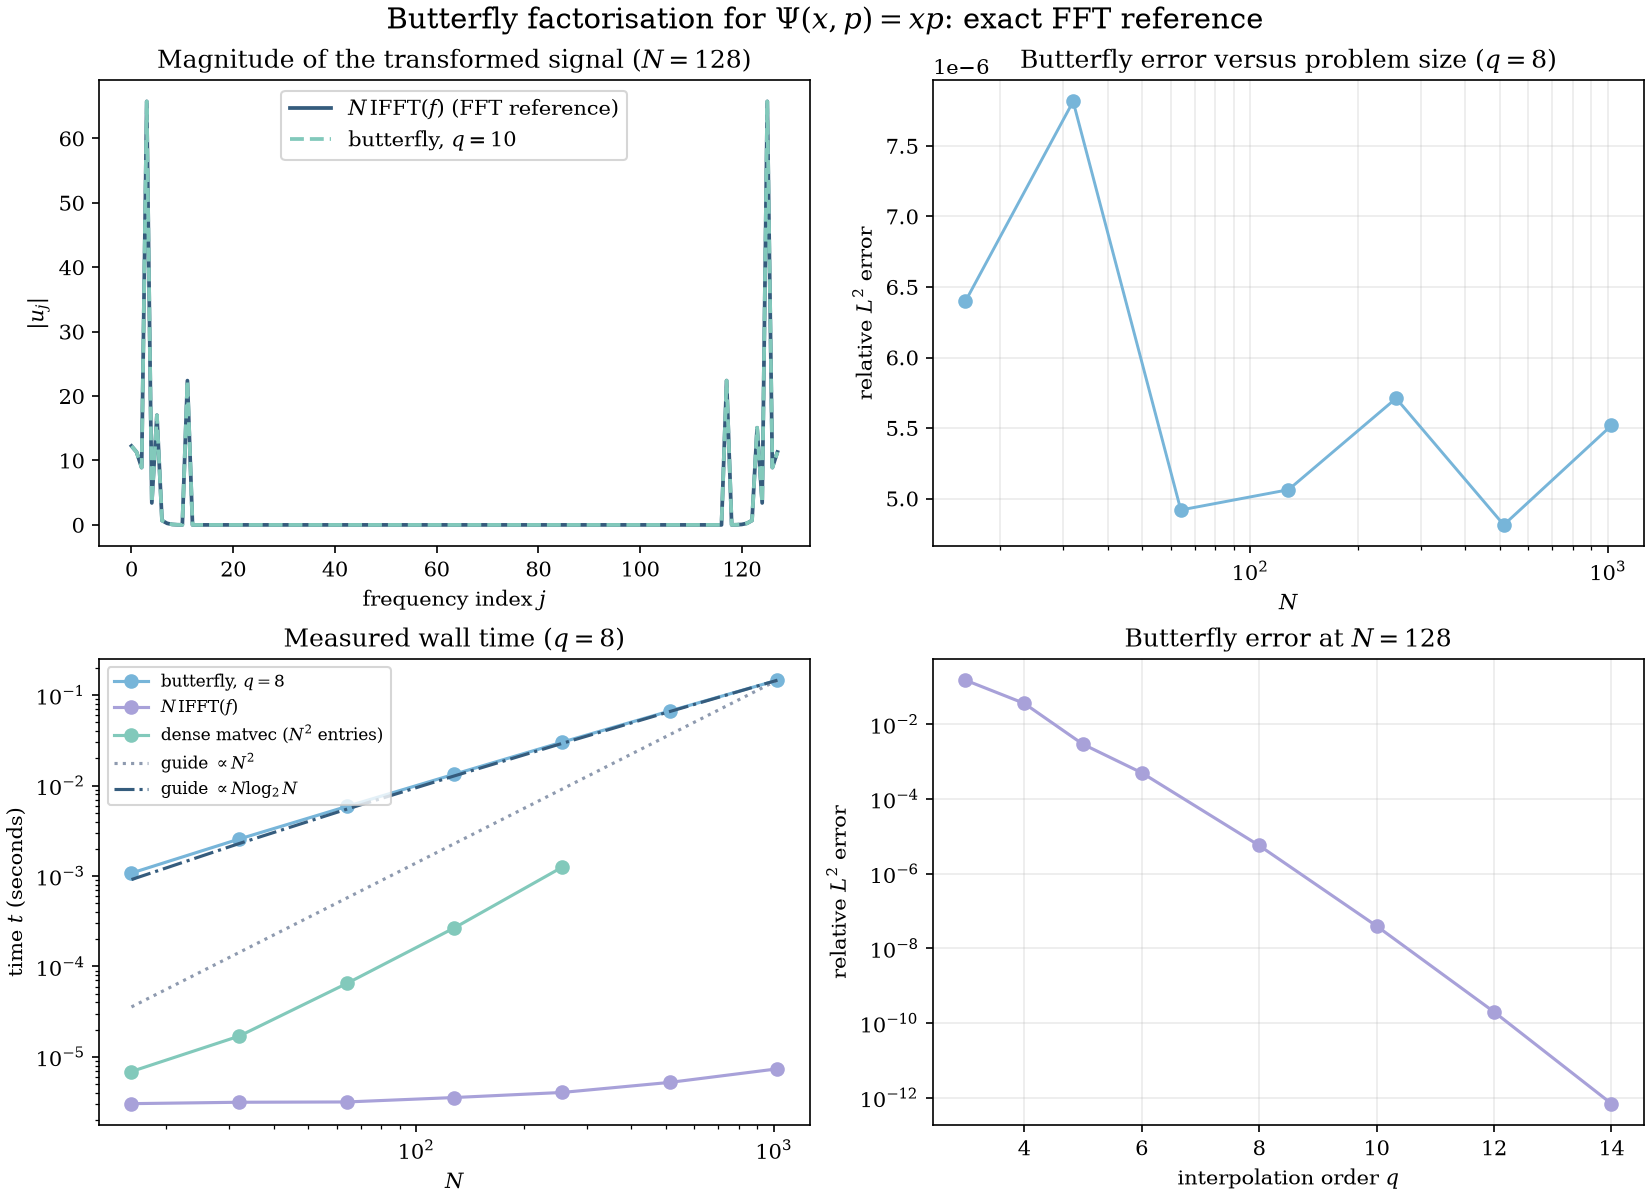
\includegraphics[width=\textwidth]{butterfly-demo/results/comparison.png}
    \caption{Comparison of the butterfly algorithm with the exact FFT reference for $\Psi(x,p)=xp$. \emph{Top left:} transformed magnitudes for a complex test signal at $N=128$, using $q=10$; the two curves are nearly indistinguishable. \emph{Top right:} relative Euclidean output error versus $N$ at fixed $q=8$, shown separately from the dependence on $q$. \emph{Bottom left:} single-thread wall times at $q=8$ for $N=16,\ldots,1024$, including a dense matrix--vector product for $N\leq256$ and guides proportional to $N\log_2N$ and $N^2$. The dense path was warmed up before timing; absolute times are machine dependent. \emph{Bottom right:} relative $L^2$ error $\|u_q-u_{\mathrm{FFT}}\|_2/\|u_{\mathrm{FFT}}\|_2$ at $N=128$ as the Chebyshev interpolation order $q$ varies. All approximation errors use $u_{\mathrm{FFT}}=N\,\operatorname{IFFT}(f)$ as the reference.}
    \label{fig:butterfly-dft-demo}
\end{figure}

\subsection{A non-DFT oscillatory example}
\label{subsec:non-dft-demo}

To check that the construction is not tied to the Fourier transform, consider
\begin{equation}
    \Psi(x,p)=xp+0.1x^2p^2.
    \label{eq:non-dft-phase}
\end{equation}
This is still real-analytic, but $R_{AB}$ is no longer simply $(x-a)(p-b)$. The explicit Taylor estimate for the bilinear example therefore does not apply; the local approximation is constructed by residual interpolation.

Figure~\ref{fig:non-dft-demo} uses this phase in the same implementation, now comparing against an explicit dense evaluation of
$Kf$, not against an FFT. The transformed magnitudes at $q=10$ agree closely, and increasing $q$ again rapidly reduces the relative Euclidean output error. This is an additional numerical test of the approximation, not a claim of a global diagonalisation or a global error estimate.

\begin{figure}[htbp]
    \centering
    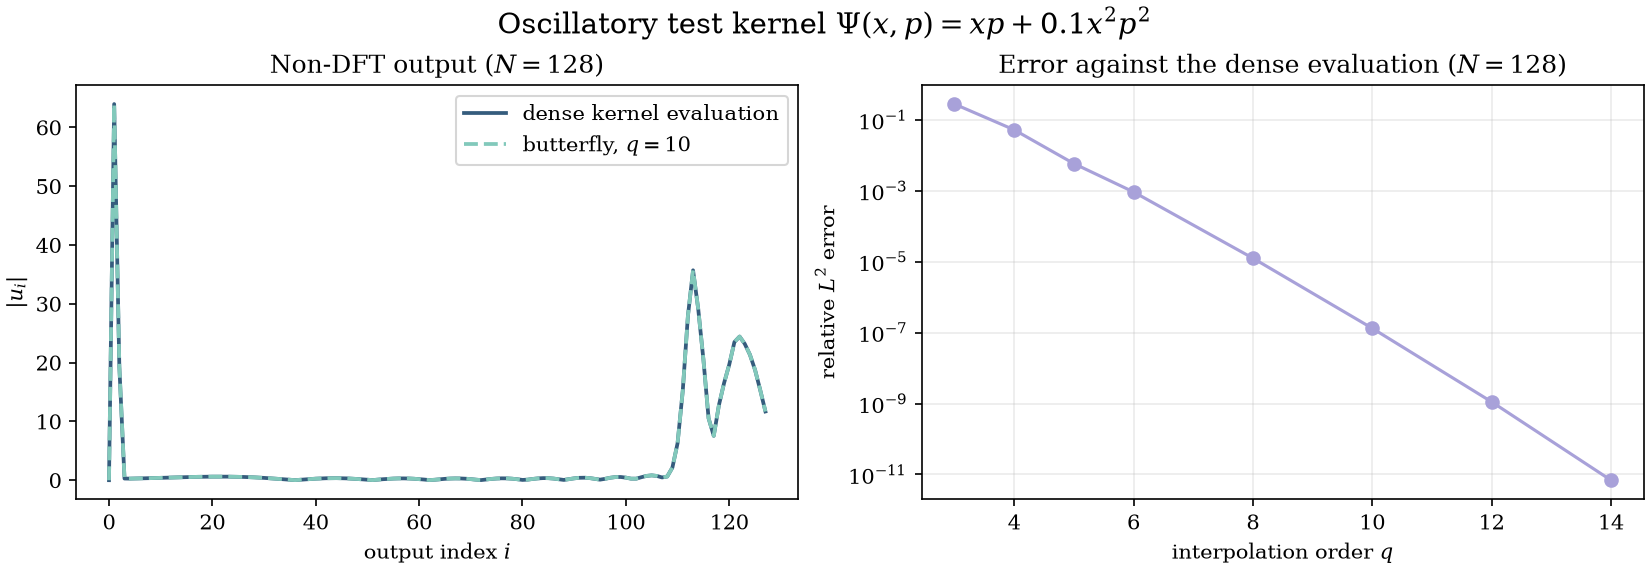
\includegraphics[width=\textwidth]{butterfly-demo/results/non_dft_comparison.png}
    \caption{Application to the non-DFT oscillatory test kernel $\Psi(x,p)=xp+0.1x^2p^2$ at $N=128$. \emph{Left:} output magnitudes from the explicit dense kernel evaluation and from the butterfly algorithm at $q=10$. \emph{Right:} relative $L^2$ error $\|u_q-u_{\mathrm{dense}}\|_2/\|u_{\mathrm{dense}}\|_2$ against the Chebyshev interpolation order $q$. Unlike the DFT comparison, the reference here is computed entirely by dense evaluation of~\eqref{eq:non-dft-phase}.}
    \label{fig:non-dft-demo}
\end{figure}

\appendix
\section{Evidence, provenance, and scope}
\label{app:evidence}

\subsection{How the main claims are supported}
The Green-function identities in Section~1 are checked directly from the derivative jump and the boundary conditions. The Fourier diagonalization, radix-2 reconstruction, discrete symbol, and sparse-stage interpretation in Section~2 follow from the displayed algebra. The centred factorisation and mixed-difference bound in Section~4 are likewise derived in the text. The analytic rank theorem and the matrix-side butterfly construction costs are explicitly cited from the literature rather than re-proved~\cite{candes2009butterfly,li2015butterfly}.

The numerical tables and figures are finite computational checks. They are not presented as proofs of general error bounds. The Section~2 script independently constructs dense matrices and the DFT, checks unitarity and the sparse-stage product, compares a recursive FFT with the dense transform, compares the FFT solve with a dense solve, and measures finite-difference error on a fixed two-mode problem. Its code and current outputs are available at \path{consolidated/examples/fft_periodic_solver.py} and \path{consolidated/results/local/}. Section~4 uses deterministic or seeded butterfly checks against a positive-sign FFT for the DFT case and against an explicit dense kernel evaluation for the non-DFT case. The implementation and measured results are in \path{butterfly-demo/}.

\subsection{Contribution, prior work, and AI assistance}
The classical algorithms and theorems belong to their original authors. The event work represented by this version is the coordinated presentation, explicit transitions between PDE structure and matrix factorisation, small teaching implementations, and numerical verification. No new complexity theorem, production solver, or literature-first claim is made.

The supplied Section~2 draft records assistance from OpenAI Codex with exposition, LaTeX, and numerical checks. Open Math OS agents assisted during the event with reading the supplied material, editing and integrating Sections~1,~2, and~4, checking derivations and references, running Python tests, and compiling this report. Mathematical claims were reviewed through direct algebra and comparison with the cited primary sources; computational claims were tied to rerunnable code and stated parameter ranges. Final mathematical review and responsibility remain with the team.

\section{Limitations of this interim version}
This report does not yet include the project's general treatment of structured factorisations (Section~3) or its numerical-linear-algebra synthesis and final discussion. The butterfly section establishes local compressibility and explains the multilevel mechanism, but it does not prove a global end-to-end error theorem for the included implementation. It also distinguishes applying an oscillatory operator from solving a linear system. Performance figures are teaching measurements on one environment, not production benchmarks.

\begin{thebibliography}{99}
\bibitem{cooley1965fft}
J.~W. Cooley and J.~W. Tukey.
\emph{An algorithm for the machine calculation of complex Fourier series}.
Mathematics of Computation \textbf{19}(90), 297--301, 1965.
\url{https://doi.org/10.1090/S0025-5718-1965-0178586-1}.

\bibitem{candes2009butterfly}
E.~J. Cand\`{e}s, L.~Demanet, and L.~Ying.
\emph{A Fast Butterfly Algorithm for the Computation of Fourier Integral Operators}.
Multiscale Modeling \& Simulation \textbf{7}(4), 1727--1750, 2009.
\url{https://arxiv.org/abs/0809.0719}.
The phase regularity hypotheses, complementary-block analysis, and explicit-kernel butterfly construction used in Section~4.

\bibitem{li2015butterfly}
Y.~Li, H.~Yang, E.~R. Martin, K.~L. Ho, and L.~Ying.
\emph{Butterfly Factorization}.
Multiscale Modeling \& Simulation \textbf{13}(2), 714--732, 2015.
\url{https://arxiv.org/abs/1502.01379}.
Matrix-side complementary low-rank conditions, nested bases, construction models, and sparse-factor complexity.
\end{thebibliography}
\end{document}
